\documentclass{article}
\usepackage{listings}
\usepackage[T1]{fontenc}
\usepackage{algorithm}
\usepackage{algorithmic}
\usepackage{amsfonts}
\usepackage{tikz}
\usepackage{systeme}
% Language setting
% Replace `english' with e.g. `spanish' to change the document language
\usepackage[polish]{babel}

% Set page size and margins
% Replace `letterpaper' with `a4paper' for UK/EU standard size
\usepackage[letterpaper,top=2cm,bottom=2cm,left=3cm,right=3cm,marginparwidth=1.75cm]{geometry}

% Useful packages
\usepackage{amsmath}

\usepackage{graphicx}
\graphicspath{ {./} }
\usepackage[colorlinks=true, allcolors=blue]{hyperref}

\title{Algorytm znajdowania sumy podzbioru}
\author{You}

\begin{document}
\maketitle

\begin{abstract}
Your abstract.
\end{abstract}

\section{Wstęp}
Problem sprawdzania czy z $n-$elementowego muiltizbioru $S$ liczb naturalnych jesteśmy w stanie wybrać podzbiór, którego suma elementów jest równa zadanej liczbie $t$ jest jednym z klasycznych problemów algorytmicznych. W nieniejszej pracy zaprezentuję niedeterministyczny algorytm opracowany przez Ce Jin i Hongxun Wu, który kożystając ze sprytnych obserwacji na polu analizy matematycznej i algebry jest w stanie podać wynik w czasie $O(n+tlog^2(t))$, co jest czasem znacznie szybszym niż klasyczny algorytm oparty na programowanie dynamiczne. 

\section{Algorytm klasyczny}

Na wejściu otrzymujemy multizbiór liczb naturalnych $S=\{s_1,s_2,...,s_n\}$, oraz 
liczbę naturalną $t$. Chcemy odpowiedzieć na pytanie czy jest możliwe wybranie 
$S' \subseteq S$ taki, że suma jego elementów jest równa $t$, przy czym wskazanie tego 
podzbioru nie jest konieczne, a wystarczy nam jedynie odpowiedź Tak lub Nie. 


Klasyczny algorytym polega na stworzeniu t-elementowej tablicy przechowującej wartości 
$0$ i $1$(dlatego najoptymalniej jest użyć do tego bitsetu). 

\begin{algorithm}
\caption{}
\begin{algorithmic}
    \STATE $create\ a\ (t+1)-element\ DP\ array\ with\ initial\ value\ of\ F$
    \STATE $DP[0] = T$
    \FOR{$i$ from $1$ to $n$}
    \FOR{$k$ from $s_i$ to $t$}
    \STATE $dp[i] = dp[i] \lor dp[k-s_i] $
    \ENDFOR
    \IF{dp[t]}
    \STATE return T
    \ENDIF
    \ENDFOR
    \STATE return F
\end{algorithmic}
\end{algorithm}

Dowód poprawności tego algorytmu jest prostym dowodem indukcyjnym, w którym teza indukcyjna
jest tezą mocniejszą i brzmi ona tak: po wykonaniu $i$-tej iteracji pętli z iteratorem $i$ $DP[m]=T$ 
wtedy i tylko wtedy
gdy można wybrać podzbiór zbioru $\{S_1,S_2,...,S_i\}$ taki, że suma jego elemetów wynosi 
$m$(oczywiście dla $k \in \{0,1,...,t\}$). 
\begin{itemize}
    \item Dla $i = 0$ teza jest oczywista.
    \item Załóżmy, że teza jest prawdziwa dla $i-1$. Jeżeli istnieje podzbiór
    zbioru $\{s_1,s_2,...,s_i\}$ taki, że suma jego elementów wynosi $k$ to jest to 
    albo podzbiór zbioru $\{s_1,s_2,...,s_{i-1}\}$ i z tezy indukcyjnej $dp[k]=T$
    jeszcze przed wykonaniem $i$-tej iteracji, albo jest to podzbiór zawierający element
    $s_i$, którego pozostałe elementy należące do $\{s_1,s_2,...,s_{i-1}\}$ sumują się 
    do $k-s_i$, więc z tezy indukcyjnej $dp[k-s_i] = T$. Ponieważ $dp[k]$ po wykonaniu $i$-tej iteracji
    przyjmuje wartość $dp[i] \lor dp[k-s_i] $ teza indukcyjna jest prawdziwa.
  \end{itemize}
Ponieważ komórki $DP$ przyjmują tylko wartości $T$ i $F$ do reprezentacji jej najoptymalniej
użyć bitsetu a kolejne iteracje pętli zewnętrznej wykonać poleceniem $dp |= (dp >> s_i)$.

Pętla zewnętrzna wykona się $O(n)$ razy i każda iteracja zajmie $O(t)$ czasu tak więc czas działania całego algorytmu zajmie $O(nt)$ i $O(t+n)$ pamięci.
\section{Idea algorytmu Ce Jin i Hongxun Wu}

Specyfikacja naszego problemu jest następująca. Na wejściu otrzymujemy liczbę $n$ będącą wielkością
zbioru $S$, $n$ liczb naturalnych będących elementami zbioru $S$ oraz nieujemną liczbę naturalną
$t$. Jeżelli wśród podzbirów $S$ istnieje taki, którego suma elemenów jest równa $t$ zwracamy 
prawdę, jeżeli zaś taki zbiór nie istnieje zwracamy fałsz.

Algorytm Ce Jin i Hongxun Wu bazuje na dość trywialnej obserwacji, że dla danego zbioru
$\{S_1,...,S_n\} \subset \mathbb{N}$ istnieje jego podzbiór sumujący się do $t \in \mathbb{N}$ wtedy 
i tylko wtedy gdy, współczynnik przy $x^t$ w  wielomianie $A(x) :=\prod_{i = 1}^{n}(1+x^{s_i})$ jest 
niezerowy. Zamiast liczyć ten współczynnik wprost najpierw obliczymy $B(x):=\ln(\prod_{i = 1}^{n}(1+x^{s_i}))$, 
zaś następnie $\exp(B(x)) = A(x)$. 

Co to jednak znaczy, że obliczymy te funkcje? Będziemy wyliczać rozwinięcia jej w szereg Taylora.
Współczynnik przy $x^t$ w rozwinięciu w szereg Taylora $\exp(B(x))$ istotnie jest współczynnikiem
przy $x^t$ w $A(x)$. Wynika to bezpośrednio z jednoznaczności rozwinięcia w szereg potęgowy. 

W dalszej części pracy będę stosował schemat notacji $F_t(x)$ jako oznaczenie rozwinięcia w szereg Taylora 
$t$-pierwszych wyrazów funkcji $F$, tak więc $exp_t(x) = \sum_{i=0}^t\frac{x^i}{i!}$, zaś 
$\ln_t(\prod)=\sum_{i=0}^t\frac{(-1)^{i-1}x^i}{n}$ 

Aby znaleźć odpowiedź na omawiany w tej pracy problem wystarczy oczywiście ustalić jedynie 
wartość $t$ pierwszych wyrazów rozwinięcia w szereg Taylora funkcji $\exp(B(x))$. 
Niestety obliczenia potrzebne do znalezienia tych współczynników mogą wymagać użycia bardzo dużych liczb długości $O(t)$. 
Obliczenia na nich mogą być więc czasochłonne. Ce Jin i Hongxun Wu skożystali z faktu, że
nie jest jedynie obiektem, który można zdefiniować analitycznie jako przekształcenie funkcji 
$f(x)$ w funkcję zwracającą dla argumentu $x$ wartość $\lim_{h \to 0}\frac{f(x+h)-f(x)}{h}$, ale 
i przekształcenie czysto algebraiczne, które przekształca szereg $\sum_{i=0}^{\infty}f_i x^i$ w
$\sum_{i=1}^{\infty}if_{i}ix^{i-1}$. 

Tak zdefiniowana pochodna zachowuje algebraiczne właściwości($f'+g'=(f+g)'$,$(fg)'=f'g+g'f$,
$(f(g))'=f'(g)g'$) bez względu na to do jakiego ciała należą współczynniki tych szeregów. 

Okazuje się, że w naszym algorytmie wystarczy rozpatrywać jedynie rozpatrywać rozwinięcia używanych 
funkcji jedynie do $t$-tego wyrazu i jeżeli weźmiemy liczbę pierwszą $p>t$ to w tym przypadku
oznacza to brak konieczności dzielenia przez liczby podzielne przez $p$, tak więc ciałem, w 
którym możemy rozpatrywać współczynniki naszych szeregów jest ciało reszt modulo $p$ dla jakiejś losowo wybranej $p>t$. Dodawanie liczb $a$ i $b$ w takim ciele przypomina dodawanie w liczbach całkowitych jednak zamiast zwracać "cały" wynik dodawania w liczbach całkowitych
zwracamy tylko jego resztę z dzielenia przez $p$. Mnożenie i odemowanie wykonuje się 
analogicznie, z kolei dzielenie przez liczbę $d$ polega na pomnożeniu przez odwrotność
$d$ w ciele $Z_p$.

W naszym algorytmie co prawda udało się uniknąć dzielenia, przez liczby podzielne przez $p$,
jednak wciąż jest możliwe uzyskanie liczb podzielnych przez $p$ na drodze dodawania i mnożenia, co może sprawić, że błędnie zinterpretujemy niektóre liczby jako $0$. W szczególności możliwe jest błędne zidentyfikowanie jako $0$ $t$-tego współczynnika wielomianu 
$A(x)$ co w bezpośredni sposób może wpłynąć na poprawność zwracanej odpowiedzi. Okazuje się
jednak, że prawdopodobieństwo takiego błędu w algorytmie Ce Jin i Honguxun Wu jest $O(n+t)^{-1}$. Ja użyłem w swojej implementacji nieco innej metody losowania tej liczby, jednak jak
eksperymentalnie sprawdziłem można zastosować dla tego sposobu analogiczny sposób szacowania prawdopodobieństwa błędu, jaki zastosowali Ce Jin i Honguxun Wu o czym więcej będę pisał w dalszej części pracy.

Ważną optymalizacją w liczeniu współczynników rozwinięcia $\exp(B(x))$ było zastąpienie jednej podwójnej pętli, której wykonanie w sposób naiwny zajmowałoby pesymistycznie $O(t^2)$ czasu pomnożeniem dwóch wielomianów stopnia co najwyżej $O(t)$, co można wykonać szybką 
transformatą Furiera. Aby uniknąć problemów z utratą dokładności w obliczeniach na liczbach 
zmienno przecinkowych zastosowałem Teorio-liczbową szybką transformatę Furiera, w której współczynniki rozpatrywałem w ciele wylosowanej już na potrzeby wcześniej omawianych obliczeń 
liczby $p$.

Ogólnie implementację algorytmu można podzielić na 5 zasadniczych części
\begin{itemize}
  \item Implementacja funkcji losującą liczbę pierwszą $p$ o porządanych własnościach
  \item Implementacja klasy odpowiadającej za wykonywanie obliczeń w ciele $Z_p$
  \item Implementacja Teorio-liczbowej szybkiej transformaty Furiera w ciele $Z_p$
  \item Implementacja algorytmu właściwego
  \item Implementacja kodu testującego, w tym algorytmu naiwnego.
\end{itemize}

\section{Szukanie liczby pierwszej}
W pracy Jin i Wu liczba pierwsza którą losujemy ma tylko jedno zastosowanie. Jest nim
wyznaczenie ciała w którym będziemy wykonywać nasze obliczenia. Losowanie to odbywa się 
zpośród liczb na przedziale $[t+1,(n+t)^3]$. Dowód oszacowania prawdopodobieństwa, 
że liczba ta nie dzieli $t$-tego współczynnika $A(x)$ jako $O(n+t^{-1})$ kożysta z tego, że
na badanym przedziale liczb pierwszych jest $\Omega((n+t)^2)$, co wynika z twierdzenia o 
liczbach pierwszych mówiącym, że $\lim_{x \to \infty} \frac{\pi(x)}{\frac{x}{\ln(x))}}=1$, gdzie $\pi(x)$ to liczba liczb pierwszych niewiększych od $x$.

Różnica, między moją implementacją, a algorytmem opisanym przez Ce Jin i Hongxun Wu jest 
jednak taka, że nie używałem klasycznej wersji szybkiej transformaty Furiera, opartej na
liczbach zespolonych, a teorio-liczbowej szybkiej transformaty Furiera wykonującej obliczenia
w ciele $Z_p$. Tak więc w tym ciele $Z_p$ musi istnieć pierwiastek z 1 stopnia $r$ gdzie
$r$ jest postaci $2^k$, dla pewnej liczby naturalnej $k$, oraz $r$ jest większe lub równe 
stopniowi wielomianu, który powstanie po pomnożeniu wielomianów, które mnożymy naszą 
transformatą powiększonego o $1$. Mnożone wielomiany są stopnia co najwyżej $t$, tak więc
możemy przyjąć, że $2^k$ to najmniejsza potęga $2$ o całkowitym wykładniku większa niż 
$2t+2$, zaś $p$ ma postać $r2^k+1$. Istotnie dla każdej liczby pierwszej $p$ istnieje jej pierwiastek pierwotny $a$,
którego stopień jest równy $p-1$, czyli w tym przypadku $r2^k$, zaś stopień tego pierwiastka podniesiony
do potęgi $r$ wynosi $2^k$.

Intuicjyjnie można przypuszczać, że ponieważ rozmieszczenie liczb pierwszych jest trudne 
do opisania prostym wzorem, to podobny procent liczb postaci $r2^k+1$ gdzie $r$ jest liczbą
naturalną z przedziału $[t+1,(n+t)^3]$ jest pierwszy, co po prostu, procent liczb 
pierwszych na przedziale $[t+1,(n+t)^3]$. Dla uproszczenia możemy badać przedział $[0,(n+t)^3]$, ponieważ $t+1$ jest względnie małe w stosunku do $(n+t)^3$. 
Ostatecznie nasza hipoteza jest taka, że jeżeli $\pi'(x)$ to liczba liczb pierwszych postaci $r2^k+1$ , gdzie $r$ jest
liczbą naturalną niewiększą od $x$. To $lim_{x \to \infty}\frac{\pi'(x)}{\frac{x}{\ln(x)}}$
jest równe $1$.

W przeciwieństwie do większości pozostałego kodu, który przygotowałem, ze względu na jednoczesne łatwe wykonywanie wykresów, oraz szybkość działania eksperymentalne weryfikowanie
tej hipotezy przeprowadziłem w języku Julia i przy użyciu programu Jupyter Notebook.

Oczywiście eksperymentalne wyznaczenie $\pi'(x)$ dla dużych $x$-ów byłoby bardzo czasochłonne więc wartość $\frac{\pi'(x)}{x}$ szaacowałem przy pomocy funkcji, która najpierw losowała $100000$
liczb typu $UInt64$ modulo $x$, mnożyłem, przez $2^k$ i dodawałem $1$, zaś następnie sprawdzałem przy pomocy funkcji
$isprime$ należącej do pakietu $Primes$ czy otrzymana 
tak liczba jest pierwsza i jeśli odpowiedź była pozytywna inkrementowałem zmienną $ans$, której 
początkowa wartość wynosiła $0$. Następnie zwracałem  $\frac{ans}{100000}$, czyli liczbę
stosunek wylosowanych liczb pierwszych do ilości losowań. Wartość $\pi'(x)$ wyliczałem dla $x$
postaci $100000000000000k+1$, gdzie $k \in \{0,1,..99\}$, oraz gdzie parametr $2^k$ jest równy
$1,2,4,8,16,64,256,1024,2^{20},2^{30}$ i $2^{50}$. Żeby uniknąć problemów z tym, że liczby
przekraczać będą limity zmiennej całkowitej $64$-bitowej bez znaku odrazu po wyliczeniu losowanej liczby
modulo $x$ rzutowałem ją na zmienną BigInt. 

Na poniższym wykresie prezentuję jak poniższa metoda pozwoliła szacować $\frac{\pi'(x)}{\frac{x}{\ln(x)}}$
(oś pionowa), w zależności od argumentu $x$(oś pionowa) i parametru $2^k$(kolor).

\begingroup
\centering
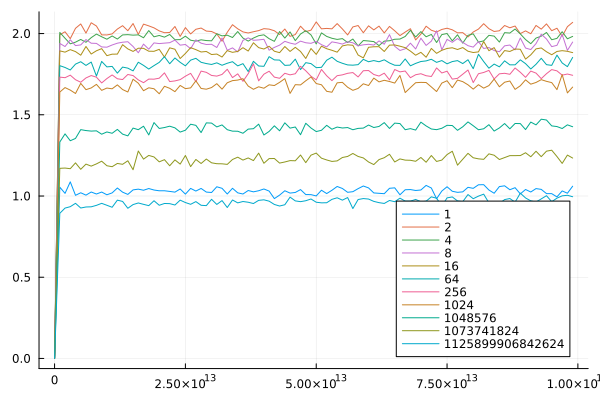
\includegraphics[width=15cm]{/home/lukasz/CLionProjects/untitled/plot1.png}
\endgroup

Jak widać z wykresu nawet dla bardzo dużych $2^k$ i $x$, wartości $\frac{\pi'(x)}{\frac{x}{\ln(x)}}$ są 
rzędu wielkości $O(1)$, co więcej dla dość małych wartości $2^k>1$ można zauważyć, że $\frac{\pi'(x)}{\frac{x}{\ln(x)}}$ jest 
większe niż $1$ i zbliżone do $2$. Zgadza się to z intuicją, że jeżeli wybieramy jedynie liczby nieparzyste,
to prawdopodobieństwo natrafienia na liczbę złożoną jest około $2$ razy mniejsze, bo "odpadają" nam 
liczby parzyste, które poza $2$ są zawsze złożone. Być może jeszcze zwiększając zakres $x$ okazałoby się, że 
że dla $2^k=2^{50}$ również badana wartość zaczęłaby się zbliżać do $2$, jednak otrzymane szacowania i tak
są już dla nas satysfakcjonujące, tym bardziej, że mnożenie wielomianów rozmiarów rzędu $2^{50}$ nawet przy pomocy
szybkiej transformaty Furiera i tak dla zdecydowanej większości współczesnych komputerów jest zadaniem niemożliwym
do wykonania w czasie, który można by nazwać "rozsądnym" a sama pamięć potrzebna do przechowania
tak dużej ilości współczynników byłaby rzędu petabajtów. 

Plik typu ipynb w którym przechchowuję kod użyty w omawianych wyżej eksperymentach znajduje się
w dołączonym do pracy repozytorium i nosi nazwę "primeExperiment.ipynb".


Omówię teraz już samą implementację modułu szukającego liczby pierwszej. Wszystkie wymienione niżej funkcje zostały 
zaimplementowane w języku C++.

Składa się on z kilku funkcji, z których zdecydowanie najprostsza jest $absolutevalue$ która
zwraca po prostu wartość bezwzględną liczby którą przyjmuje jako argument. Służy ona po prostu
łatwemu pozbyciu się problemu z tym, że niektóre liczby losowane przez używaną w dalszej
części kodu funkcję $rand()$ liczby mogą być ujemne, podczas gdy iteresują nas tylko liczby dodatnie. 
Druga bardzo prosta funkcja to funkcja $pow2$ która dla przyjmowanej jako argument liczby $t$ 
zwraca najmniejszą potęgę $2$ z wykładnikiem naturalnym, która jest większa niż $t$. Jest to po prostu
mnożenie przez $2$ zmiennej $ans$ której początkowa wartość jest równa $1$ dopóki nie będzie 
większa niż $t$. Musimy wykonać co najwyżej $63$ mnożenia, co jest na tyle szybkie, że nie ma 
potrzeby stosowania jakiś bardziej zaawansowanych algorytmów jak na przykład 
używających algorytm szybkiego potęgowania.

Funkcja $randomLongLong$ służy losowaniu liczby 64-bitowej niewiększej niż podana jako argument 
liczba $mod$. Należąca do standardu C++ funkcja $rand$ zwraca liczby 32-bitowe, co może nie być dla nas
wystarczające. Jeżeli $mod<2^{31}$ zwracam po prostu resztę z dzielenia przez $mod$ wartości bezwzględnej
wyniku wywołania $rand()$. Jeżeli zaś jest ona większa niż $2^{31}$ najpierw pobieramy jej 31 
najmniej znaczących bitów z wylsowanej liczby $candidate1$, zaś następnie losujemy liczbę 
całkowitą $candidate2$ z przedziału $[0,\frac{mod}{2^{31}}]$.
Potem łączymy obie liczby wyliczając wartość $candidate2 \cdot 2^{31}+candidate1$ co jest faktycznie 
losową liczbą z zadanego przedziału.

Kolejną nieco bardziej złożoną funkcją jest funkcja $isprime$ sprawdzającą czy podana jako argument 
liczba $x$ jest pierwsza. Jeżeli $x \leq 1$ oczywiście zwracamy fałsz. Jeżeli zaś jest równe $2$ zwracamy
prawdę. Jeżeli jest liczną parzystą większą niż $2$ zwracamy fałsz. Następnie zmienną $i$ o początkowej wartości $3$ 
iterujemy się po kolejnych licznach nieparzystych dopóki zachodzi warunek $i \cdot i \leq x$.
Jeżeli $i$ dzieli $x$ przerywamy iterację i zwracamy fałsz. Jeżeli zaś zakończymy omawianą pętlę przed zwróceniem fałszu
zwracamy prawdę. Istotnie liczba nieparzysta złożona musiałaby mieć dzielnik nieparzysty mniejszy lub równy jej
pierwiastkowi kwadratowemu. Niepokoić może fakt, że musimy w pesymistycznym przypadku wykonać $O(\sqrt{x})$ iteracji.
W praktyce jednak nawet jeżeli $x$ jest bardzo duże, zbliżone do górnego zakresu zmiennych typu $long$ $long$ 
wykonanie tej funkcji zajmuje najwyżej kilka sekund, a ponieważ zdecydowana większość liczb złożonych ma 
dość mały najmniejszy dzielnik pierwszy to, w praktyce o ile liczba podana na wejście nie jest pierwsza, dla nawet bardzo dużych $x$ szybko przerwiemy wykonanie omawianej pętli i nie będzie konieczności czekać nawet tych kilku sekund.

Kolejną już ostatnią funkcją w tym module jest funkcja $find\_prime$. Przyjmuje ona jako argumenty liczbę $n$ i $t$, zaś następnie zwraca liczbę pierwszą postaci $r2^k+1$, gdzie $r$ jest liczbą naturalną z przedziału $[t+1,(n+t)^3]$. Na początku przy pomocy funkcji $pow2$ wyznaczam $2^k$. Następnie losuję potencjalne liczby $r$ modulo $(n+t)^3$, przy pomocy
funkcji $randomLongLong$. Jeżeli wylosuję liczbę niewiększą niż $t$ losuję jeszcze raz. Dla zwłaszcza dużych $n$ i $t$
prawdopodobieństwo tego jest znikome, a nawet jeśli się zdaży, to czas powtórzenia losowania jest znikomy. Następnie mnożę
wylosowane $r$ z wyznaczonym $2^k$ i dodaję do wyniku $1$. Kolejnym krokiem jest dla tak uzyskanej liczby sprawdzenie, czy 
jest pierwsza przy pomocy funkcji $isprime$. Niepokoić może, koniczność wykonywanie niewiadomej ilości losowań i sprawdzeń, pierwszości wylosowanych liczb. Warto jednak zauważyć, że oczekiwana liczba losowań wynosi $O(\log(n+t))$ i większość przypadków sprawdzania złożoności liczb złożony zachodzi bardzo szybko, bo bardzo szybko w funkcji $isprime$ znajdujemy jej dzielnik pierwszy(na przedziale $[0,N]$ dla dużych $N$ zaledwie nieco ponad $0.08$ liczb ma dzielnik pierwszy większy niż 1000000 co szybko może sprawdzić poniższy krótki skrypt w Julii:
\begin{lstlisting}
zans=1
for 3 in 1:1000000
    if isprime(i)
        ans *=(i-1)
        ans /= i
    end 
    println(ans)
end
\end{lstlisting}
Kod funkcji omówionych w tej sekcji znajduje się w pliku $find\_prime.h$.

\section{Implementacja ciała $Z_p$}
Ogólny szablon, jakie metody należy zaimplementować był 
mocno inspirowany implementacją klasy dużych liczb całkowitych
zamieszczony na stronie [ https://www.geeksforgeeks.org/bigint-big-integers-in-c-with-example/ ]


Ponieważ praktycznie wszystkie(poza rzeczami typu zwiększanie iteratora) będziemy wykonywać na elmentach ciała
$Z_p$ w którym istnieją operatory działań arytmetycznych, aby uniknąć ciągłych konieczności pobierania ekxlicite
wartości modulo $p$ z wyników działań najwygodniejszym podejściem byłoby zaprogramowanie klasy $field$ której instancje
reprezentują elementy ciała $Z_p$ zaś przeciążone operatory odpowiadają działaniom w $Z_p$ i pisząc bardziej 
wysokopoziomowe funkcje nie musimy już się troszczyć o to, by jakkolwiek "nromalizować" wyniki. 

Jednym z pól naszen klasy jest zmienna typu $long$ $long$ i nazwie $p$. Jest to po prostu wartość liczby $p$ 
modulo którą wykonujemy obliczenia. Metoda $setP$ ustawia wartość
$p$ na przyjętą jako argument wartość zmiennej $x$ tylu 
$long$ $long$. Ustawia również zmienną $m$ na wartość $(LONG\_MAX / p)$, jednak jej
zastosowanie omówię w dalszej części pracy. Zmienna $p$ jest zawsze taka 
sama dla wszystkich instancji klasy możemy uczynić ją zmienną statyczną(podobnie jak dokładniej 
omawianą w dalszej części m).

Pole, które przechowuje wartość pojedynczego obiektu nazwałem value. Oczywiście
pole te już nie może być statyczne.
Stworzyłem kilka konstruktorów dla klasy $field$. Konstruktor domyślny
nie przyjmuje żadnego argumentu i ustawia wartość $value$ na $0$. 
Konstruktor kopiujący ustawia wartość $value$ na wartość $value$ obiektu 
typu $field$ podanego jako argument. Ostatnie dwa konstruktory
przyjmują jako argument liczbę całkowitą $val$ odpowiednio typu
$int$ i $long$ $long$ i ustawiają wartość pola $value$ na resztę z
dzielenia $val$ przez $p$ jednak ponieważ dla uproszczenia chcemy trzymać
jako $value$ tylko liczby nieujemne zamiast przypisać polu $value$ wprost
wartości $val \% p$, przypisujemy jej wartość $((val\%p)+p)\%p$ co jak 
można łatwo stwierdzić w istocie zawsze przyjmuje wartość dodatnią będącą
resztą z dzielenia $val$ przez $p$.

Przejdę teraz do omówienia kolejnych funkcji i przeciążonych operatorów
w omawianej klasie.

Funkcja  getValue służy pobraniu wartości zmiennej $value$, która ma 
ustawioną prywatność na $default$.

Metody $field$ $inline$ $\&operator++()$, 
$field$ $inline$ $operator++(int temp)$,
$field$ $inline$ $\&operator--()$,
$field$ $inline$ $operator--(int temp)$ to odpowiednio przeciążenia
operatora postinkrementacji, preinkrementacji, postdekrementacji i predekrementacj.
Operator postinkrementacji kożystając z niezmiennika, mówiącego,
że wartość pola $value$ jest zawsze liczbą całkowitą z
przedziału $[0,1,..,p-1]$ który
zachowują wszystkie funkcje modyfikujące pole $value$ oraz konstruktory
może przypisać w miejsce $value$ po prostu wartość wyrażenia
$(value+1)\%field::p$. Ponieważ jeżeli $value=0$ naiwna postdekrementacja
powoduje uzyskanie wyniku ujemnego zamiast $(value+1)\%field::p$ w przypadku
postdekrementacji przypisujemy zmiennej $value$ wartość
wyrażenia $(field::p+value-1)\%field::p$. Dla operatora 
preinkrementacji najpierw tworzymy zmienną $aux$ w której przechowujemy
starą wartość obiektu, którą później zwrócimy, a następnie na oryginalnym 
obiekcie dokonujemy zdefiniowaną wcześniej postinkrementację.
Operator predekrementacji definiujemy analogicznie jak preinkrementacji.

Następnie definiuję przeciążenia operatorów $+=,+,-=,-$. Operator
$+=$ przyjmuje przez referencje dwa argumenty typu $field$,
gdzie pierwszy oznaczam jako $a$, zaś drugi jako $b$. Wartości pola
$value$ przypisujemy wartość $( a.value + b.value ) \%field::p$ gdzie 
operator $\%$ służy zachowaniu niezmiennika, by wartości pola $value$
były mniejsze niż $p$. Z kolei dla operatora $-=$ wartości analogicznego
pola przypisujemy wartość wyrażenia $(a.value-b.value+field::p)\%field::p$
gdzie nieobecne w poprzednim przypadku dodanie $p$ służy niedopuszczeniu
do sytuacji gdy $value$ stanie się ujemne jeśli $b.value > a.value$.
W implementacji operatora $+$ tworzymy zmienną tymczasową temp, o wartości
początkowej pola $value$ takiej samej jak $a.value$, a następnie
przy pomocy zdefiniowanego wcześniej operatora $+=$ dodajemy do tego obiektu
obiekt $b$. Analogicznie definiujemy operatora $-$;

Kolejnymi nieco prostszymi operatorami jakie zdefiniowałem to operatory porownójące
$==,!=,<,<=,>=,>$, które dla argumentów $a$ i $b$ po prostu zwracają wartości boolowskie odpowiednio 
wyrażeń $a.value == b.value$, $a.value != b.value$, $a.value < b.value$, 
$a.value <= b.value$, $a.value >= b.value$ i $a.value > b.value$.

Nieco bardziej skomplikowana jest implementacja operatora $*=$. Ponieważ liczba 
$p$ mnoże być rzędu $O((n+t)^3)$ to gdybyśmy postąpili naiwnie i (przyjmując 
oznaczenie pierwszego argumentu jako $a$, drugiego jako $b$) przypisali odpowiedniemu
polu wartość wyrażenia $(a.value*b.value)\%field::p$ wynik mnożenia $a.value*b.value$
byłby rzędu $O((n+t)^6)$, co już dla $n+t$ rzędu $10^3$ mogłoby powodować wychodzenie poza zakres 
zmiennej $long$ $long$. Oczywiście tak mały zakres liczb mocno wpłynąłby na użyteczność
zaimplementowanych przezemnie programów. Definiuję więc zmienną $m$, będącą 
górną wartością $b$, dla którego możemy wykonać mnożenie w sposób naiwny (i następnie 
wyciągnąć tylko resztę z dzielenia przez $p$) bez obaw o przepełnienie. W 
przeciwnym wypadku tworzę zmienną pomocniczą $A$ będącą wartością pola value
obiektu $a$ oraz zmienną $B$ będącą wartością pola value obiektu $b$.
Zauważmy, że $A \cdot B = A \cdot \lfloor \frac{B}{m} \rfloor \cdot  + A \cdot (B \% m)$
Wartość $m$ jest zależna od $p$ i dlatego ustawiamy ją podczas operacji $setP$ o czym pisałem w 
jednym poprzednich akapitów. Najpierw rekurencyjnie używając $*=$ mnożę
obiekt typu $field$ o wartości zmiennej $value$ równej $A$ przez obiekt $field(B/m)$ i wynik 
trzymam w obiekcie $ans1$, zaś następnie tworzę obiekt $field ans2 = field(A*(B\%m))$(żeby 
wartość $value$ dla tak powstałego obiektu była z odpowiedniego zakresu "pilnuje" definicja konstruktora).
Do zmiennej $a$ zapisuję wynik dodawania tych obiektów.

Kolejnym operatorem jest operator $*$. Argumenty, które otrzymuje
to obiekty typu $field$ o nazwach $a$ i $b$. Tworzę tymczasową zmienną $temp$
o tej samej wartości co $a$ i następnie mnożę ją przez $b$ przy pomocy
zdefiniowanego wcześniej operatora $*=$ i zwracam tak zmodyfikowany obiekt $temp$.

Kolejnym operatorem jest operator potęgowania $\textsuperscript{$\wedge$}=$. Pierwszym argumentem jaki przyjmuje 
jest obiekt typu $field$ o nazwie $a$ oraz zmienna typu $long$ $long$ o
nazwie $b$. Zauważmy, że z małego twierdzenia Fermata $a^{p-1} \equiv 1 (\mod p) $, tak więc
zamiast podnosić $a$ do potęgi $B$ możemy podnieść ją do potęgi $B\%(p-1)$.
Teoretycznie moglibyśmy rozpatrywać $((b\%(p-1))+p-1) \% (p - 1)$, jednak z pewnych powodów, o 
których napiszę w dalszej części zdecydowałem się rozpatrzeć przypadki $B$ ujemnego i 
dodatniego osobno. 

Jeżeli $b==0$ przypisuję $a$ wartość $1$ i zwracam wynik. Jeżeli $B$ = 1 nie 
nie robię nic, tylko odrazu zwracam $a$. Jeżeli $B==-1$ to jeżeli $a.value==0$ 
wyrzucam błąd dzielenia przez $0$, jeżeli zaś nie robię następującą procedurę.
Ponieważ potęgowanie do $-1$ to znalezienie odwrotności $a$ w $Z_p$
z małego twierdzenia Fermata oznacza to podniesienie $a$ do potęgi 
$p-2$. Potęgowanie można zaimplementować, by wykonywać się w czasie logarytmicznym
względem liczby mnożeń, jednak mnożenie ze względu na groźbę przepełnienia
też może w pesymistycznym przypadku zabierać logarytmicznie dużo czasu.
Znalezienie odwrotności obiektu jest dość podstawową operacją, którą 
możemy chcieć wykonywać dość często, tak więc czas $O(\log ^2(p))$ może
nie być zadowalający. Dlatego klasa $field$ posiada jeszcze jedno pole, którym
jest statyczna mapa o nazwie $inverse$ z wejściami typu $<long$ $long,long$ $long>$, która przypisuje 
liczbie $x$ liczbę która jest wartością pola $value$ odwrotności $field(x)$. Tablicę tą 
czyścimy, za każdym razem gdy zmieniamy wartość $p$. Istotnie wtedy odwrotności
tych samych liczb mogą stać się inne, bo zmienia się ciało w którym są tymi odwrotnościami.
Operacja $insertInverse$ przyjmuje zmienne typu $field$, które zakładamy
explicite, że są elementami wzajemnie odwrotnymi i oznaczamy jako $a$ oraz $b$, 
a następnie, jako, że $(a^{-1})^{-1}=a$ wykonujemy od razu 2 przypisania
\begin{lstlisting}
  field::inverse[a.value] = b.value;
  field::inverse[b.value] = a.value;
\end{lstlisting}
Gdy mamy wyliczyć potęgę o wykładniku $-1$ jakiegoś elementu $a$ typu $field$ sprawdzam 
najpierw czy w mapie odwrotności jest przypisana wartość dla klucza $a.value$(nie jest
przypisana wtedy i tylko wtedy gdy wartością wyrażenia $field::inverse[a.getValue()] == 0$ jest
prawda), a następnie jeżeli kluczowi temu przypisana jest wartość ustawiamy $a.value$ na nią i zwracamy $a$, zaś
jeżeli nie wykonujemy operację $field::insertInverse(a, A\textsuperscript{$\wedge$}=(( long long)(field::p-2)))$
(gdzie rekurencyjnie wywołujemy operastor $\textsuperscript{$\wedge$}=$ dla wartości nieujemnej)
i ponownie pobieramy wartość dla klucza $a.value$. Pozwala nam to dla każdego elementu $Z_p$ wyliczyć
jego odwrotność co najwyżej raz, bez względu na ilość wywołań tego wyliczenia w wyżej poziomowym 
kodzie. 

Kolejnym przypadkiem, który należy rozważyć to gdy $B>1$. Zauważmy, że $a^b=a^{\lfloor\frac{B}{2} \rfloor} \cdot a^{\lfloor\frac{B}{2} \rfloor} \cdot a$
jeżeli $B$ jest nieparzyste lub $a^B=a^{\lfloor\frac{B}{2} \rfloor} \cdot a^{\lfloor\frac{B}{2} \rfloor}$ jeżeli $B$ jest parzyste.
Tworzę więc pomocnicze obiekt $a0$ o tej samej wartości pola $value$ co $a$. Rekurencyjnie
wykonuję $a0 =\textsuperscript{$\wedge$} (B/2)$. Kolejne wykonania $a0 =\textsuperscript{$\wedge$} (B/2)$
mają drugi argument mniejszy lub równy $\frac{1}{2}$ poprzedniego drugiego argumentu, więc ilość 
tych wywołań nim drugi argument będzie równy $0$ lub $1$ jest $O(log(B))$. Następnie mnożymy obiekt $a0$ przez
samego siebie przy pomocy operatora $*=$, i teraz aktualna wartość $a0$ wynosi 
$a^{\lfloor \frac{B}{2}\rfloor} \cdot a^{\lfloor \frac{B}{2}\rfloor}$. Jeżeli $B$
jest nieparzyste mnożymy przy pomocy $*=$ $a$ przez $a0$, jeżeli zaś jest parzyste 
po prostu przypisujemy obiektowi $a$ wartość obiektu $a0$. W obu przypadkach zwracamy $a$.

Kolejnym i już ostatnim przypadkiem jest gdy $B < -1$. W tym przypadku wykożystujemy 
fakt, że $a^B=(a^{-1})^{-B}$. Tak więc kolejno wykonujemy zdefiniowane wcześniej 
podniesienie $a$ do potęgi $-1$ przy pomocy operatora $\textsuperscript{$\wedge$} =$ a następnie znów przy
pomocy tego samego operatora podnosimy $a$ do potęgi $-B>1$, co też zostało już wcześniej
zdefiniowane. Po wykonaniu tych obliczeń zwracam $a$.

Kolejnym operatorem jest $\textsuperscript{$\wedge$}$. Pobiera on argument $a$ typu field i $b$ typu $long$ $long$, tworzy
przy pomocy konstruktóra kopiującego tymczasowy obiekt $temp$ typu $field$ z taką samą wartością pola 
$value$ co $a$, następnie przy pomocy operatora $\textsuperscript{$\wedge$}=$ podnosi 
$temp$ do potęgi $B$ i zwraca tak zmodyfikowaną wartość $temp$.

Kolejnym operatorem będzie operator dzielenia $/=$ przyjmujący dwa argumenty typu 
$field$ oznaczone odpowiednio jako $a$ i $b$. Dzielenie w ciele modulo nie oznacza
"klasycznego" dzielenia arytmetycznego, ale pomnożenie przez element odwrotny. Tak więc tworzymy nowy obiekt $B$ będący kopią $b$ i mnożymy $a$ przy pomocy
operartora $*=$ przez $B\textsuperscript{$\wedge$}(long$ $long)(-1)$. Następnie zwracamy tak zmodyfikowane $a$.

Kolejnym operatorem jest $/$. Otrzymuje on dwa argumenty typu $fieled$ o nazwach $a$ i $b$. Tworzę obiekt $temp$ typu field i przypisuję mu wartość $a$, następnie dzielę przez $b$ przy pomocy 
operatora $/=$ i zwracam $temp$.

Kolejnym operatorem jest operator wczytania ze strumienia wejściowego $>>$.
Jako argument otrzymuje strumień (obiekt typu
$std::istream$) oraz obiekt typu $field$ o nazwie $a$.
Funkcja mu odpowiadająca najpierw wczytuje ze strumienia $in$ wartość tymczasowej zmiennej $s$ typu $long$ $long$
a, następnie przypisuje obiektowi $a$ wartość $field(s)$. Następnie zwracam strumień $in$.

Kolejnym już ostatnim operatorem jest wypisanie obiektu typu field na strumień wyjściowy
$<<$. Jako argument pobiera strumień wyjściowy (obiekt typu $std::ostream$) o nazwie $out$ oraz 
obiekt typu $field$ i nazwie $a$. Funkcja mu odpowiadająca wypisuje po prostu wartość pola 
$a.value$ na strumień $out$ i zwraca ten strumień. 

Omówiony w powyższej sekcji kod został napisany w języku $C++$ i znajduje się w 
pliku $field.h$ w dołączonym do pracy repozytorium.

\section{Teorio-liczbowa szybka transformata Furiera}

Dyskretna transformata Furiera jest służy przyspieszeniu mnożenia wielomianów. Idea algorytmu jest następująca. Idea algorytmu jest następująca. Chcemy pomnożyć wielomiany(reprezentowane jako wektor współczynników)$A(x)$ i $B(x).$Zamiast liczyć naiwnie wartości współczynników $AB$ najpierw obliczamy wartości wielomianów $A$ i $B$ w punktach których liczba jest większa lub równa stopniowi $AB$, a następnie mnożymy 
wartości w tych samych punktach, wyznaczając wartości $AB$ w nich. Ponieważ liczba punktów
przekracza stopień $AB$ wyznacza jednoznacznie ten wielomian i z tych obliczonych wartości możemy szybko wyznaczyć wartości współczynników $AB$. 

Wybór punktów opiera się na prostej obserwacji, że jeżeli $A(x) = a_0x^0+a_1x^1+..+a_{2n-1}x^{2n-1}$
(jeżeli stopień $A$ ma stopień parzysty przyjmujemy po prostu, że $a_{2n-1}$ jest równe $0$). jest równe
sumie $A_0(x^2)$ gdzie $A_0(t)$ jest równe $\sum_{i=0}^{n-1}a_{2n}t^{i}$, oraz 
$A_1(x^2)x$, gdzie $A_1(t)$ jest równe $\sum_{i=0}^{n-1}a_{2n+1}t^{i}$. Tak więc jeżeli dwie
liczby $a$ i $b$ mają te same wartości swoich kwadratów możemy obliczyć tylko raz wartości $A_1$ i $A_2$
od tego kwadratu, a następnie w czasie stałym połączyć te wyniki, tak aby uzyskać wartości 
wielomianu $A$ w punktach $a$ i $b$. 


Klasyczna wersja dyskretnej transformaty Furiera oblicza wartości wielomianu $A$ dla
argumentów z ciała liczb zespolonych. Przyjmujemy następujące oznaczenie $A(x)=\sum_{i=0}^{\infty}a_ix^i$,
przy czym istneie $I$ takie, że $\forall i>I: a_i = I$. I oznaczając dalej 
 $A_0(x) = a_0x^0+a_2x^1+..+a_{2^m-2}x^{2^{m-1}-1} $
oraz $A_1(x) = a_1x^1+a_3x^1+..+a_{2^m-1}x^{2^{m-1}-1} $, przy czym $2^m$ jest najmniejszą
potęgą $2$ o wykadniku naturalnym, większym niż stopień wielomianu będącego wynikiem optymalizowanego 
przez nas mnożenia. 

Będę oznaczał $\omega_m$ jako $e^{\frac{i2\pi}{2^m}}$. 
Zaóważmy, że :
\begin{equation*}
  \systeme{
  A(\omega_m^1) = A_0(\omega_m^2)+A_1(\omega_m^2)\omega_m^1 = A_0(\omega_{m-1}^1)+A_1(\omega_{m-1}^1)\omega_m^1,
  A(\omega_m^2) = A_0(\omega_m^4)+A_1(\omega_m^4)\omega_m^2 = A_0(\omega_{m-1}^2)+A_1(\omega_{m-1}^2)\omega_m^2,
  A(\omega_m^6) = A_0(\omega_m^6)+A_1(\omega_m^6)\omega_m^3 = A_0(\omega_{m-1}^3)+A_1(\omega_{m-1}^3)\omega_m^3,
  \cdot \cdot \cdot ,
  A(\omega_m^{2^m}) = A_0(\omega_m^{2^{m+1}})+A_1(\omega_m^{2^{m+1}})\omega_m^{2^m} = A_0(\omega_{m-1}^{2^m})+A_1(\omega_{m-1}^{2^m})\omega_m^{2^m}}
\end{equation*}

Tak więc gdy mamy wektory $V_0=\Bigl( A_0(\omega_{m-1}^0),A_0(\omega_{m-1}^1),...,A_0(\omega_{m-1}^{2^{m-1}})\Bigr)$ oraz                          

$V_1=\Bigl( A_1(\omega_{m-1}^0),A_1(\omega_{m-1}^1),...,A_1(\omega_{m-1}^{2^{m-1}})\Bigr)$ możemy
w czasie liniowym wyliczyć wektor $V=\Bigl( A(\omega_{m}^0),A(\omega_{m}^1),...,A(\omega_{m}^{2^{m}})\Bigr)$, jednak wektory 
$V_1$ i $V_2$ można znów rozbić na wyliczenie najpierw $2$ wektorów długości $2^{m-2}$ i 
połączenia tych dwóch wektorów w czasie liniowym od ich długośći. Możemy tak rozbijać kolejne wektory, aż dojdziemy do wektorów długości
$2$ które przechowują wartości pewnych wielomianów $0$-stopnia będący po prostu jednym ze współczynników $A$.
 Niech $O(t)$ będzie czasem 
policzenia wartości wielomianu $A$ w $n=2^m$ punktach przy pomocy dyskretnej transformaty Furiera. 
Furiera. Wiemy, że $O(t)=2O(\frac{t}{2})+O(n)$. Rozwiązaniem takiego równania jest $O(t)=O(n\log(n))$.
Okazuje się, że po wyliczeniu wartości wielomianów u $AB$ w omawianych punktach możemy "wyciągnąć" z tych wartości w czasie
$O(n)$ wartości współczynników wielomianu $AB$, gdzie $n$ to ilość tych punktów.

Moja implementacja kożysta z dwóch klasycznych ulepszeń dyskretnej transformaty Furiera. 

Pierwsza to tak zwana "Teorio-liczbowa transformata Furiera". Polega ona na nie wykonywaniu obliczeń w ciele $C$ lecz
w $Z_p$, przy czym istnieje oczywiście musi istnieć pierwiastek z $1$ stopnia $2^m$, gdzie $2^m$ jest potęgą $2$ o wykładniku
naturalnym i większa niż stopień zwracanego wielomianu. Pierwiastek ten też podniesiony do jakiejkolwiek potęgi 
o wykładniku naturalnym dodatnim, mniejszym niż $2^m$ musi być różny od $1$. 
Tak naprawdę oznacza to po prostu, że $p$ ma postać $r2^m+1$, gdzie $r$ jest liczbą nauralną, o czym pisałem w poprzedniej 
sekcji.

Drugim ulepszeniem jest użycie tak zwanego szybkiej transformaty Furiera. Opiera się na obserwacji że rekurencyjna wersja dyskretnej transformaty Furiera opiera
się na najpierw podzieleniu współczynników wielomianu na coraz mniejsze grupy, aż do pojedynczego współczynnika, a następnie łączeniu pojedynczych współczynników
w pary zawieerające informację o $2$ współczynnikach, potem czwórki, ósemki, aż gdy połączymy je w jeden blok, zawierający informacje o wszystkich współczynnikach, a rekurencyjne wywołania służą jedynie pogrupowaniu
w jakiej kolejności będziemy wykonywać łączenia.
 
Możemy jednak to grupowanie wykonać bez rekurencyjnego wywoływania transformaty po prostu ustawiając obok siebie współczynniki w takiej kolejności odpowiadającej 
tak aby pary indeksów $(0,1)$, $(2,3)$,...,$(2^m-1)$ odpowiadały polom w wektorze łączonych w pierwszej fazie łączenia iteracji, $(0,1,2,3)$,
$(4,5,6,7)$, $(8,9,10,11)$,...,$(2^m-4,2^m-3,2^m-2,2^m-1)$ w drugiej, itd. 

Przejdźmy do dokładnego opisu naszej implementacji. 

Najpierw definiuję funkcję $enoughGoodRoot$ która przyjmuje liczbnę $k$ typu $long$ $long$ i zwraca element typu $field$ na którym aby był równy 
$1$ trzeba wykonać dokładnie $k$ podniesień jej do kwadratu. Na początku deklaruję zmienną $powerof2$ typu $long$ $long$ będącą
największą potęgą $2$ o wykładniku naturalnym takim, że dzieli on zmienną statyczną $p$ klasy $field$ pomniejszoną o $1$, którą definiowałem
w poprzedniej sekcji. Liczbę tą wyznaczam przez przypisanie jej początkowej wartości równej $1$, i mnożeniu jej w pętli przez $2$
dopóki wartość wyrażenia $(field::p-1)/powerof2$ nie będzie liczbą nieparzystą. Następnie tworzymy zmienną $odd$ typu $long$ $long$ będącą po 
prostu liczbą po której pomnożeniu przez $powerof2$ i dodaniu $1$ otrzymyujemy $field::p$. Wiemy, z małego twierdzenia Fermata, że każda liczba względnie 
pierwsza z $field::p$ podniesiona do $2^{powerof2}odd$ przystaje do $1$ modulo $field::p$. Dalsza część algorytmu polega na losowaniu niezerowego obiektu klasy $field$ o nazwie $candidate$,
podniesieniu go w miejscu do potęgi $odd$, a następnie sprawdzeniu ile razy tak uzyskany obiekt należy podnieść do kwadratu, nim będzie on równy $1$. W tym celu podnosimy w pętli do kwadratu
kopię $candidate$ i póki nie dojdziemy do $1$ inkrementujemy zmienną $funnyLog$, która początkowo jest równa $0$ i po wykonaniu omawianej pętli ma ona wartość równą liczbie tych podniesień do kwadratu. Jeżeli $funnyLog$ jest większe niż $k$ (zakładamy, że $2^k<powerof2$) to liczba powstała przez podniesienie $candidate$ do kwadratu $funnyLog-k$ razy
jest naszym szukanym pierwiastkiem. Jeżeli tak nie jest losujemy do skutku nowego $candidate$, jednak za każdym razem prawdopodobieństwo
sukcesu jest nie mniejsze niż $\frac{1}{2}$, bo z prawdopodobieństwem $\frac{1}{2}$ wylosujemy nieresztę kwadratową $field::p$. (ZRODOLOOO ZNALEZC!!!!!!!!!!!!!!!!!!!!).

Kolejnym etapem jest odpowiednie ustawienie wartości w komórkach wektora ze współczynnikami wielomianu(nazwę go $coefficients$), tak by można było wykonać na niej iteracyjną wersję szybkiej transformaty
Furiera. Okazuje się, że należy je uszeregować w takim porządku, że wartość znajdująca się w polu $coefficients[n]$ musi znaleźć
się w polu $reverseBits(n,k)$, która oznacza zmienną powstałą po odwróceniu $k$ ostatnich bitów zmiennej $n$, gdzie 
$2^k$ to ilość pól wynikowego wektora. Funkcja $reverseBits$ składa się z klasycznego algorytmu odwócenia kolejności bitów 
zmiennej, polegającym na najpierw zamianie ze sobą dwóch sąsiednich bitów przy pomocy operatorów $|$, przesunięć bitowych
i wyzerowaniu odpowiednich bitów przy pomocy operatora $\&$ i odpowiednich masek bitowych, następnie podobnej zamieniam sąsiednie bloki
po $2$ bity, następnie $4$, $8$, $16$ i $32$. Potem koryguję wynik przesówając go bitowo o $64-k$ bitów w lewo i wtedy tak uzyskaną zmienną zwracam jako wynik funkcji.

Gdy mamy już funkcję $reverseBits$ możemy stworzyć funkcję $setToDo$ transformującą wektor współczynników w "surowej" formie w wektor gotowy
do wyliczenia jego szybkiej transformaty Furiera. Jako argumenty dla tej funkcji otrzymujemy wektor elementów typu $field$ o nazwie $coefficients$ oraz
zmienną $long$ $long$ o nazwie $size$ oznaczającą rządaną długość wektora wynikowego(tak naprawdę jest to odpowiednio duża potęga dwójki o wykładniku naturalnym). Na początku dopełniamy wektor $coefficients$ elementami równymi $field(0)$ do rozmiaru $size$. Następnie w pętli z $iteratorem$ i przechodzącym po wszystkich liczbach naturalnych od $0$ do $size-1$ i jeżeli $reverseBits(i,\log_2(size)) > i$(warunek ten służy temu, by każdy element został zamieniony dokładnie raz, zauważmy też, że $reverseBits( reverseBits (i ,\log_2(size)),\log_2(size))=i$) zamieniam w tabeli pole o indeksie $i$ z polem o indeksie 
$reverseBits (i ,\log_2(size))$ miejscami. Funkcja nic nie zwraca, a jedynie modyfikuje wektor podany jako argument.

Przejdźmy do funkcji $DFT$, która otrzymując wektor współczynników wielomianu $coefficients$, liczbę $size$ nie mniejszą niż długość tego wektora i będący potęgą $2$ o wykładniku naturalnym oraz obiekt omegaM typu $field$, który jest pierwiastkiem z $1$ stopnia $size$ takim, że podniesiony do jakiejkolwiek liczby naturalnej mniejszej niż size nie jest równy $0$ zwracamy wektor zawierający wartości tego wielomianu w punktach kolejno $omegaM^0$, $omegaM^1$,...,$omegaM^{size}$. 

Na początku przygotowywujemy wektor do wykonania dalszej części obliczeń wywołując zdefiniowaną w poprzednim paragrafie funkcję $setToDo$ na wektorze $coefficients$ i dla liczby $size$. 

Tworzymy stos na który kładziemy wyniki kolejnych złożeń podniesiania do kwadratu liczby $omegaM$ aż do $-1$.

Póki stos nie będzie pusty będę w każdej iteracji pętli $while$ ściągał z niego kolejne wartości i przypisywał je do zmiennej $currentOmegaM$.
Przyjmijmgy oznaczenie, że na początku $i-tej$ iteracji wektor $coefficients$ ma postać $\frac{size}{2^{i-1}}$ bloków postaci
$(f_{i,j,0}(\omega_i^0),f_{i,j,1}(\omega_i^1),...,f_{i,j,2^{i-1}-1}(\omega^{2^{i-1}-1}_i))$. gdzie $j$ to numer bloku. Chcemy następujące po sobie pary bloków połączyć w jeden blok postaci $(f_{i+1,k,0}(\omega_{i+1}^0),f_{i+1,,1}(\omega_{i+1}^1),...,f_{i+1,j,2^{i}-1}(\omega^{2^{i}-1}_{i+1}))$, przy czym $f_{i+1,j,1}(\omega_{i+1}^k) = f_{i,2j,1}(\omega_{i}^\frac{k}{2})+f_{i,2j+1,1}(\omega_{i}^{\frac{k}{2}})\omega_{i+1}^k$. 

Każda iteracja głównej pętli zawiera 



 
\end{document}
